%
%
%
%
\chapter{Event Selection} \label{ch:event_selection}

Searching for a heavy photon resonance requires both the accurate 
reconstruction of the QED trident invariant mass spectrum and the efficient 
rejection of Bethe-Heitler events.  With this in mind, a scheme 
was developed to select events with $e^+e^-$ pairs whose kinematic signatures
resemble that of QED tridents which, in turn, mirror the kinematics of 
heavy photon production and decay.  Once a sample of QED tridents has been selected, 
additional kinematic 
requirements were applied to reject Bethe-Heitler events.  The  $e^+e^-$ events
which satisfied all criteria were used to produce the final invariant mass 
spectrum employed to search for a heavy photon resonance.  The following chapter
will discuss the selection used to arrive at the final event sample.   


\section{Data}

%%%%%%%%%%%%%%%%%%%%%
%   Table of Data   %
%%%%%%%%%%%%%%%%%%%%%
\begin{table}[h!t]
    \centering
    \begin{tabular}{ccc}
        \toprule
        \textbf{Run Number} 
        & \textbf{10\%$\times$Total Events (M)} 
        & \textbf{10\%$\times$Luminosity (nb$^{-1}$)} \\
        \midrule
        \midrule
        5723 & 10.68765  & 3.927681901  \\
        5724 & 11.397637 & 4.229082832    \\
        5725 & 8.612363  & 3.193363425   \\
        5739 & 8.0932    & 2.956111602   \\
        5741 & 10.97741  & 3.987840806   \\
        5742 & 11.174619 & 4.224543485   \\
        5743 & 6.040229  & 2.244021498 \\
        5766 & 9.927829  & 3.337962213 \\
        5769 & 11.179994 & 4.059284573 \\
        5771 & 11.642768 & 4.254619178 \\
        5772 & 11.865312 & 4.403638304 \\
        5773 & 13.429284 & 5.014898695 \\
        5775 & 5.580172  & 1.988647799 \\
        5776 & 8.121968  & 2.997741852 \\
        5782 & 12.396243 & 4.552604162 \\
        5783 & 12.226626 & 4.548117122 \\
        5791 & 10.58427  & 3.716081116 \\
        5795 & 8.789774  & 3.17431154 \\
        5796 & 12.055927 & 4.323879491 \\
        5797 & 10.047503 & 3.584285692 \\ 
        \bottomrule
    \end{tabular}
    \caption{List of ``golden'' runs from the 2015 Heavy Photon Search 
             Engineering Run used in this analysis along with the total number
             of events and luminosity of the unblinded portion of the data.}
    \label{tab:data}
\end{table}

The data used for this analysis consist of the unblinded portion of the 2015 
HPS engineering run.  This amounts to 74.72 nb$^{-1}$ (.4671 mC of charge) or 
1/10 of a PAC day.  For comparison, the projected limits shown on Figure 
\ref{fig:ap_limits} were set assuming a full PAC week (37.5 mC) of data.
The list of runs used in this analysis along with the unblinded number of 
events and luminosity for each run are shown on Table \ref{tab:data}.

\section{Event Selection}

The HPS ``pairs1'' trigger was designed to trigger on events with two clusters
whose positions in the Ecal were consistent with an $e^+e^-$ from either a trident 
reaction or the decay of an $A'$. As such, only ``pairs1'' trigger events
were considered for the final data sample.  Furthermore, only events where the
bias of the SVT was on, the SVT was positioned at 0.5 mm from the beam and 
were free of data acquisition errors were included in the data sample.

\subsection{Cluster Pair Selection}

The acceptance of the HPS detector is optimized such that the $e^+e^-$ pairs
produced in either a QED trident reaction or from the decay of an 
$A'$ are observed through their energy depositions in the Ecal.  The energy
depositions or clusters are expected to be in opposite Ecal volumes i.e. 
top/bottom and coincident in time within a coincidence window of a few ns.  This
can be seen from Figure \ref{fig:cluster_times_2d}, which plots  
cluster time of one cluster composing a pair versus the 
other.  From the figure, it can be seen that most cluster pairs of interest are 
coincident to within a few ns. Furthermore, the majority of coincident clusters
have a cluster time between $\sim$ 40 - 48 ns which corresponds approximately
to the size of the trigger window (see Figure \ref{fig:cluster_times}). 
%%%%%%%%%%%%%%
%   Figure   %
%%%%%%%%%%%%%%
\begin{figure}[t]
    \centering
    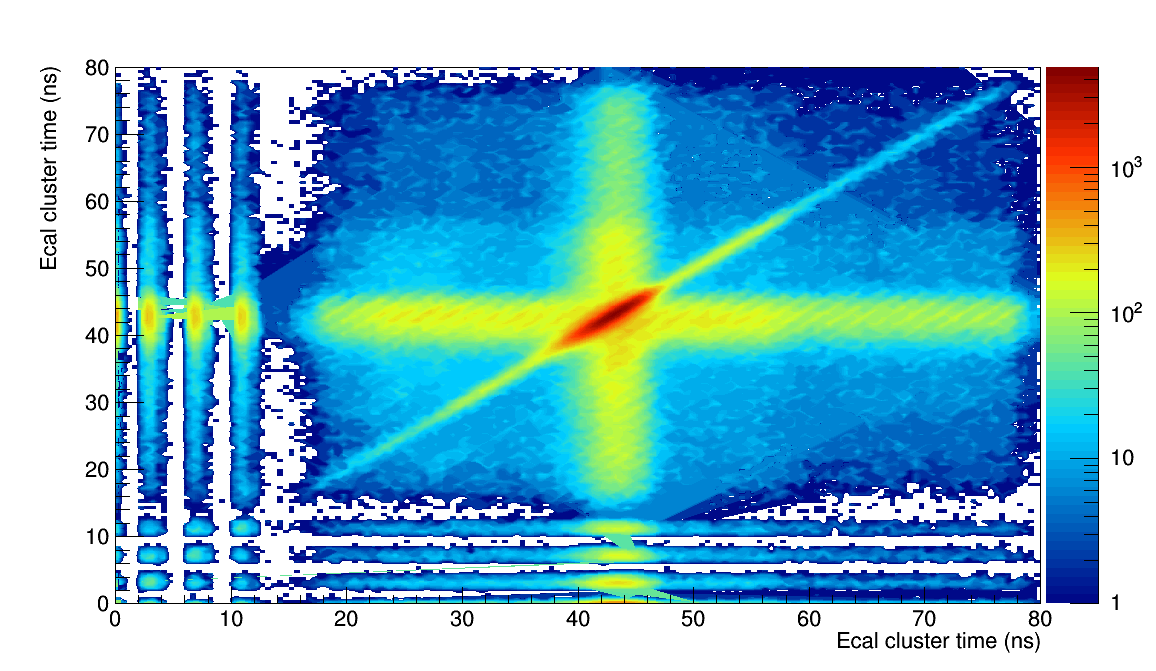
\includegraphics[width=\textwidth]{images/20160428_pass4_cluster_time_v_cluster_time.png}
    \caption{The spectrum of Ecal cluster times of one cluster composing a pair 
             versus other.  The figure clearly shows that most coincident pairs 
             fall within tight coincidence and cluster time windows.}
    \label{fig:cluster_times_2d}
\end{figure}  
%%%%%%%%%%%%%%
%   Figure   %
%%%%%%%%%%%%%%

In order to select true coincidences, the clusters forming a pair were 
required to have a cluster time between 42 ns and 47.5 ns.  Clusters outside 
of this window tend to be associated with pile-up in the calorimeter 
and fall outside of the 8 ns trigger window.  As a result, the efficiency of
finding a track associated with a cluster dramatically drops for clusters 
outside of this window. The selection is
shown graphically in red on Figure \ref{fig:cluster_times}.  Clusters satisfying
the cluster time criteria are then formed into pairs.  The difference between the
cluster time of the pair is then required to fall within a 3.2 ns window around the 
coincidence peak located at 0.003 ns (Figure \ref{fig:coin_time}).  If an event
contains multiple ``good'' cluster pairs, the pair with the smallest difference 
in time is chosen. 
%%%%%%%%%%%%%%
%   Figure   %
%%%%%%%%%%%%%%
\begin{figure}[ht]
    \centering
    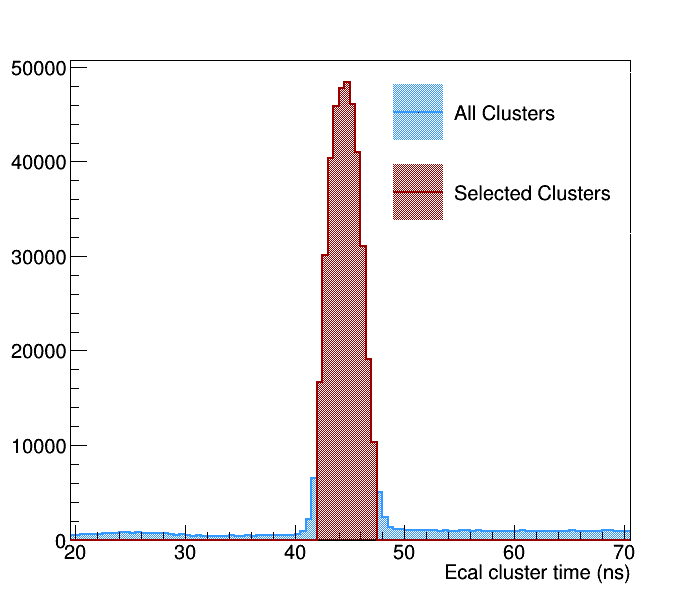
\includegraphics[width=.9\textwidth]{images/20160428_ecal_cluster_time.png}
    \caption{Cluster time of all Ecal clusters in an event (blue). The time of 
             cluster is required to be between 42 ns and 47.5 ns (red) in order to 
             ensure that it falls within the trigger window.}
    \label{fig:cluster_times}
\end{figure}  
%%%%%%%%%%%%%%
%   Figure   %
%%%%%%%%%%%%%%

%%%%%%%%%%%%%%
%   Figure   %
%%%%%%%%%%%%%%
\begin{figure}[h!t]
    \centering
    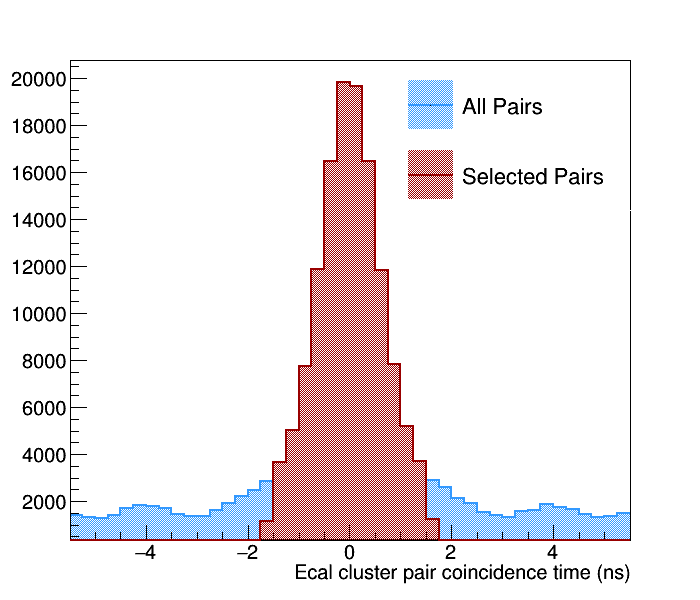
\includegraphics[width=.9\textwidth]{images/20160428_coincidence_time.png}
    \caption{The difference in time of a cluster pair in an event.  Pairs 
             selected for the final event sample are required to have a 
             difference in time that falls within a 3.2 ns window centered at 
             0.003 ns.}
    \label{fig:coin_time}
\end{figure}  
%%%%%%%%%%%%%%
%   Figure   %
%%%%%%%%%%%%%%
 
\subsection{Track-Cluster Matching}

\begin{figure}[t!h]
    \begin{subfigure}{.5\textwidth}
        \centering
        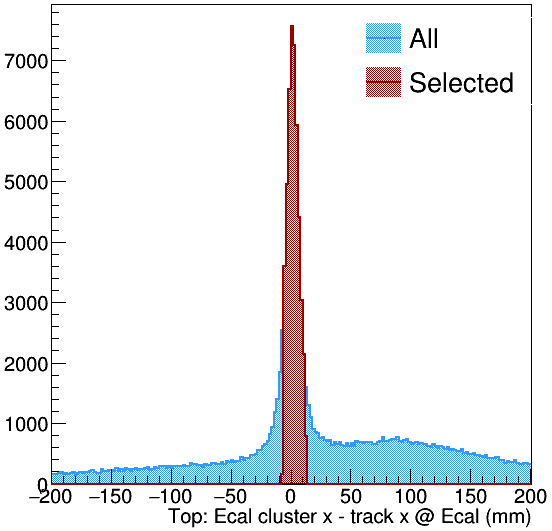
\includegraphics[width=0.85\textwidth]{images/20160502_pass4_cluster_track_delta_x_top.png}
    \end{subfigure}
    \begin{subfigure}{.5\textwidth}
        \centering
        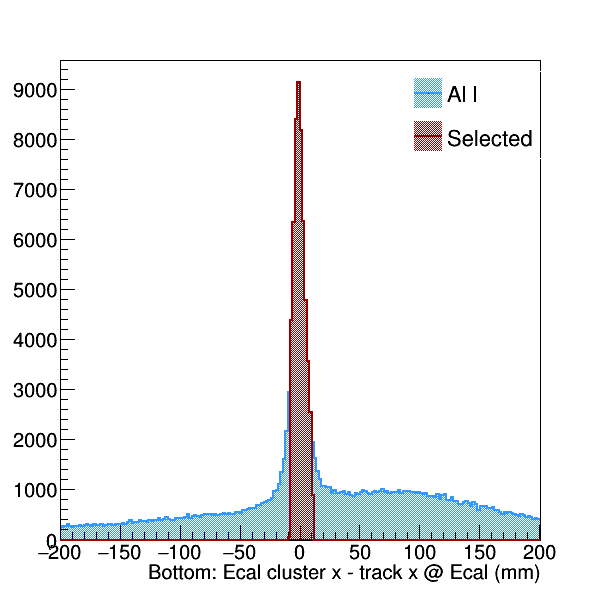
\includegraphics[width=0.85\textwidth]{images/20160502_pass4_cluster_track_delta_x.png}
    \end{subfigure}
    \caption{Difference between the $x$ position of an Ecal cluster and the 
             extrapolated track $x$ at the Ecal for all tracks and clusters in 
             an event (blue) separate by top (left) and bottom (right) detector
             volumes.  True track-cluster matches appear as a peak 
             above mismatches.  In order for a track and cluster to be considered
             a match, the difference in $x$ was required to fall within a 3$\sigma$
             window around the peak.}
    \label{fig:track_cluster_delta_x}
\end{figure}

In order to further suppress accidental coincident pairs where one or both
clusters can be attributed to a photon, the 
selected ``good'' cluster pairs are required to have tracks associated 
with them. The trajectories of all tracks in an event are propagated downstream
to the face of the Ecal using the full 3D magnetic field map.  A track and a cluster
are considered a match if the difference between their positions in both $x$ 
and $y$ satisfy the criteria listed on Table \ref{tab:track_cluster_cuts}. The 
cuts were chosen such that they create a 3$\sigma$ window around the peak of 
the cluster-track position difference distributions. The resulting selection is 
highlighted in red on 
Figure. \ref{fig:track_cluster_delta_x} and \ref{fig:track_cluster_delta_y}.
\begin{figure}[h]
    \begin{subfigure}{.5\textwidth}
        \centering
        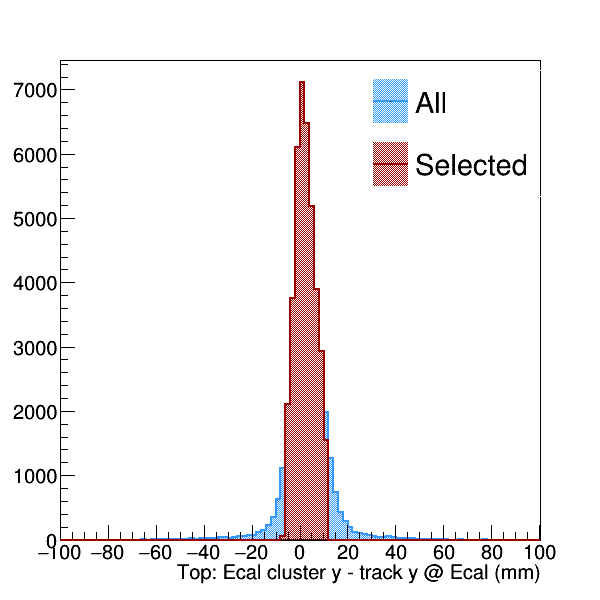
\includegraphics[width=0.85\textwidth]{images/20160502_pass4_cluster_track_delta_y_top.png}
    \end{subfigure}
    \begin{subfigure}{.5\textwidth}
        \centering
        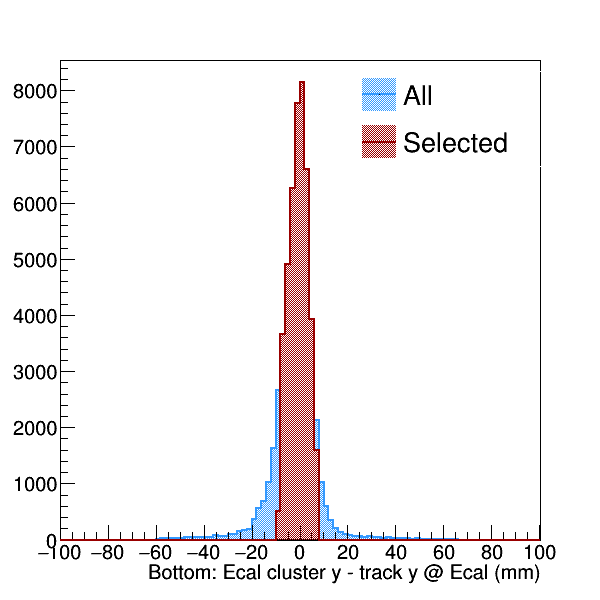
\includegraphics[width=0.85\textwidth]{images/20160502_pass4_cluster_track_delta_y_bottom.png}
    \end{subfigure}
    \caption{Difference between the $y$ position of an Ecal cluster and the 
             extrapolated track $y$ at the Ecal for all tracks and clusters in 
             an event (blue) separate by top (left) and bottom (right) detector
             volumes.  True track-cluster matches appear as a peak 
             above mismatches.  In order for a track and cluster to be considered
             a match, the difference in $y$ was required to fall within a 3$\sigma$
             window around the peak.}
    \label{fig:track_cluster_delta_y}
\end{figure}
\begin{table}[h!b]
    \centering
    \resizebox{\textwidth}{!}{
        \begin{tabular}{r|cc}
            \toprule
            & \textbf{Cluster $x$  - track $x$ at Ecal (mm)} 
            & \textbf{Cluster $y$  - track $y$ at Ecal (mm)}  \\
            \midrule
            \midrule
            Top     & $-6.10 \le x \le 12.93$ & $-6.08 \le y \le 11.49$ \\ 
            Bottom  & $-8.02 \le x \le 10.84$ & $-8.31 \le y \le 7.40$  \\ 
            \bottomrule
        \end{tabular}
    }
    \caption{Boundaries used to denote the 3$\sigma$ window used to establish if 
             an Ecal cluster and SVT track are matched to each other.  Due to 
             global misalignments, different windows are needed for top and 
             bottom tracks and clusters.}
    \label{tab:track_cluster_cuts}
\end{table}
If multiple tracks were found to match to a single cluster, the track 
with the minimum radial distance to the cluster was chosen.  


%%%%%%%%%%%%%%
%   Figure   %
%%%%%%%%%%%%%%
\begin{figure}[h!t]
    \centering
    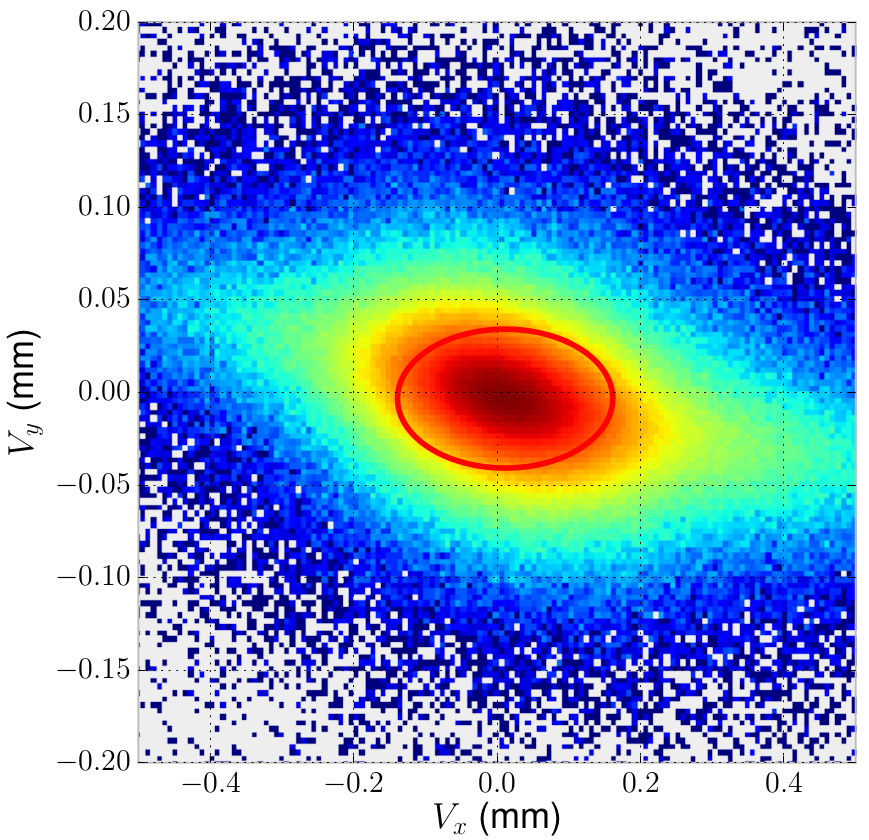
\includegraphics[width=.9\textwidth]{images/20160503_vertex_xy.png}
    \caption{Vertex position at the target of all $e^+e^-$ track pairs.  The
             elliptical selection (in red) is used to select pairs for the 
             final event sample.}
    \label{fig:vertex_xy}
\end{figure}  
%%%%%%%%%%%%%%
%   Figure   %
%%%%%%%%%%%%%%

\subsection{Final Trident Sample}

The event selection criteria that have been applied thus far only select 
events that have QED trident or $A'$ like signatures i.e. two coincident clusters that
passed the trigger cuts and have $e^+e^-$ tracks associated with them.  However, 
there remain $e^+e^-$ accidental coincidences that need to be removed from the final 
event sample.  This is best accomplished by subjecting the tracks associated 
with the clusters to the following additional criteria:
\begin{itemize}
    \item For simplicity, events that have multiple positron tracks are not 
          considered.
    \item In order to cut down on the number of misconstructed tracks that may
          have been mismatched to a cluster, both tracks are subjected to 
          $\chi^2$ probability cut of 95\%.
    \item Some electrons in the cluster pair may actually be a multiple
          Coulomb scattered beam electron of energy 1.056 GeV 
          instead of one associated with a true $e^+e^-$ 
          pair.  To remove these events from the final event sample, the 
          momentum of electron tracks are required to be less than 0.85 GeV.
    \item The $e^+e^-$ tracks associated with the clusters are vertexed with 
          their position along the beamline, $v_z$, constrained to the target. 
          For true $e^+e^-$ pairs, the vertex position in x and y ($v_x$ and $v_y$) should be
          well constrained to an ellipse with dimensionality close to the beam 
          spot.  With this in mind, the fitted vertex $\chi^2$ is first required 
          to be less than 10.  The positions along x and y are then required 
          to lie within an ellipse 
          defined as
          \[
          \left (\frac{v_x - 0.0113}{0.15} \right)^2 + \left(\frac{v_y + 0.0033}{0.05} \right)^2  \le 1.
          \]
          The elliptical selection is shown graphically on Figure \ref{fig:vertex_xy}.
\end{itemize}

%%%%%%%%%%%%%%
%   Figure   %
%%%%%%%%%%%%%%
\begin{figure}[ht]
    \centering
    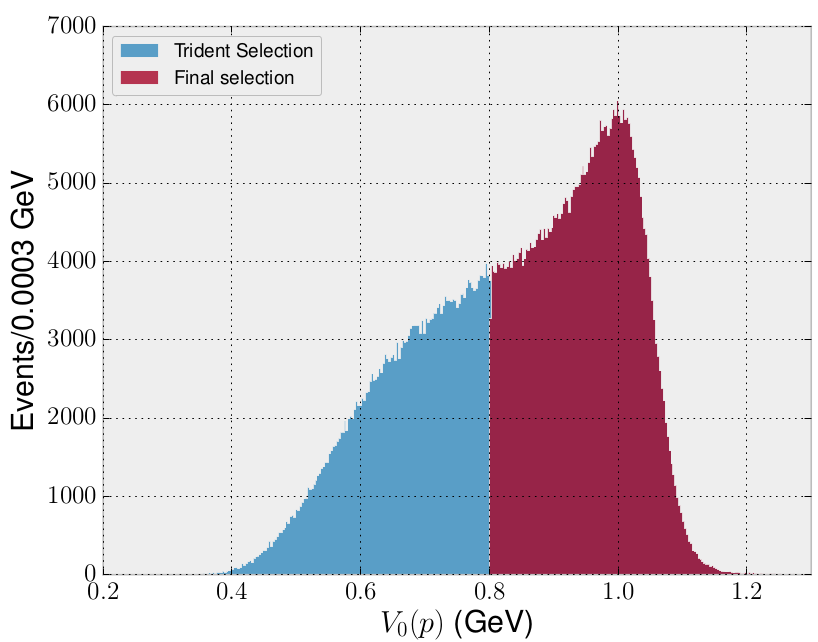
\includegraphics[width=\textwidth]{images/20160504_psum.png}
    \caption{Distribution of the sum of $e^+e^-$ momentum.  The distribution in 
             red graphically indicates the selection used to reduce the number
             of Bethe-Heitler from the final event sample.}
    \label{fig:p_sum}
\end{figure}  
%%%%%%%%%%%%%%
%   Figure   %
%%%%%%%%%%%%%%

\subsection{Radiative Selection}

As discussed in Section \ref{sec:tri_bkgs}, the kinematic similarities between
heavy photons and
radiative processes can be used to analyze both the rate of $A'$ signal production
and the sensitivity of the experiment to $A'$ signals.  It is then crucial to
maximize the fraction of radiative events in the final event sample.  The final
event sample is expected to be dominated by the Bethe-Heitler process.  However,
as discussed in Section \ref{sec:tri_bkgs}, 
the kinematic difference between the radiative and Bethe-Heitler processes can 
be exploited to reduce the number of Bethe-Heitler events.  Specifically, the 
$e^+e^-$ pair produced in a radiative process will be highly boosted, while 
only one of the electrons in the Bethe-Heitler process will be boosted 
while the other will be much softer.  With this in mind, the sum of the momentum
of the electron and positron, ``p-sum'', allows the discrimination between the two processes.
Specifically, radiative events are expected to have a ``p-sum'' peaked 
closed to the beam energy (1.056 GeV), while the distribution of Bethe-Heitlers will be peaked a 
low p-sum.

Figure \ref{fig:p_sum} shows the distribution of the sum of the momentum (p-sum) 
of the $e^+e^-$ tracks composing a pair.  Reducing the dominant Bethe-Heitler 
background was accomplished by  requiring the p-sum of 
the $e^+e^-$ tracks be greater than 0.8 GeV. 
%Using pure radiative and full trident Monte Carlo, requiring a pair to have a 
%p-sum cut greater than 0.8 GeV was found to maximize the radiative fraction.
The cut is shown graphically on Figure \ref{fig:p_sum}.

The invariant mass
distribution before (blue) and after (red) the p-sum cut was applied is shown
on Figure \ref{fig:mass_selection}.  The invariant mass distribution in red 
will serve as the starting point for the resonance search.
The details of the resonance search will be given in Chapter \ref{chap:resonance}.

\begin{figure}[t]
    \centering
    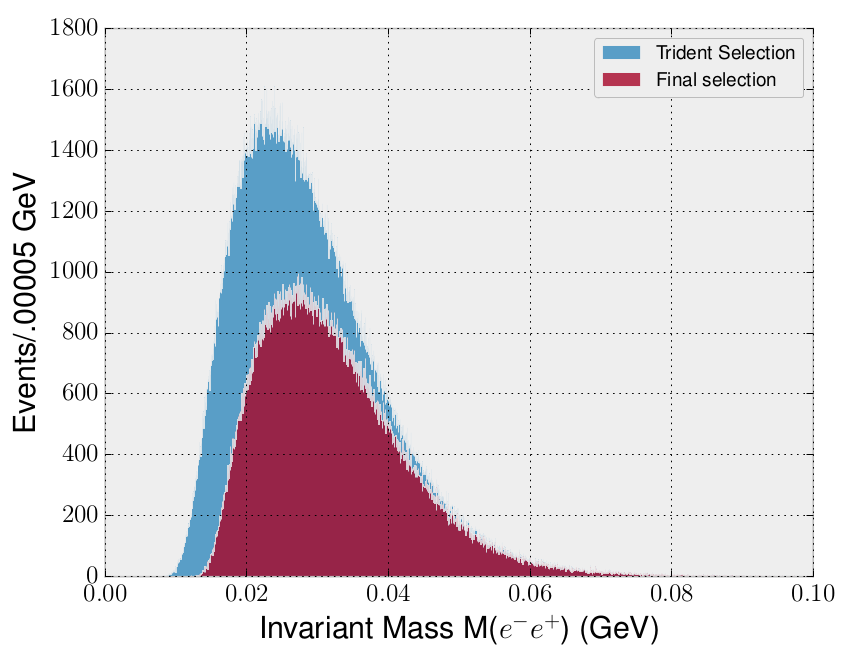
\includegraphics[width=1.0\textwidth]{images/20160504_invariant_mass_selection.png}
    \caption{The Heavy Photon Search $e^+e^-$ invariant mass distribution before (blue) 
             and after (red) a cut on the sum of the $e^+e^-$ momentum. 
             The mass distribution in red 
             will serve as the starting point for the resonance search.}
    \label{fig:mass_selection}
\end{figure}

\subsection{Event Selection Efficiency}

The cuts used to select the final invariant mass distribution along with their
selection efficiency for data, trident monte carlo (MC), pure radiative 
monte carlo and 50 MeV A' events are summarized on Table \ref{tab:sel_eff}.
The trident MC sample used contains both Bethe-Heitler and radiative events.

\begin{sidewaystable}
    \centering
    \begin{tabular}{l||c|c|c|c|c}
        \toprule
        \textbf{Description of Cuts} 
        & \multicolumn{2}{c|}{\textbf{Data}}
        & \textbf{Trident MC}
        & \textbf{Radiative MC}
        & \textbf{50 MeV A' MC} \\
        \midrule
        \midrule
        & N$_{\text{events}}$ & $\varepsilon$ (\%)
        & $\varepsilon$ (\%) 
        & $\varepsilon$ (\%)
        & $\varepsilon$ (\%) \\ 
        \midrule
        \midrule
        Pair 1 Trigger Count & 162825923 & -  & - & - & - \\
        Single positron & 12705660 & 7.80  & 75.05 & 70.73 & 85.90 \\
        Good cluster pair & 4529997 & 2.78  & 51.10 & 54.60 & 73.74 \\
        Track-cluster match & 1735394 & 1.07  & 21.11 & 27.19 &55.49 \\
        Track $\chi^2 < 15$ &1236300  & 0.76  &17.33  & 21.66 &32.52  \\
        $e^-$ momentum $ < 0.85$ GeV & 1194117 & 0.73  & 17.31 & 21.63 &32.48  \\
        Vertex $\chi^2 < 10$ and elliptical &710558  & 0.44  &13.36  & 15.86& 23.67 \\
        $e^+e^-$ momentum sum $<$ 0.8 GeV & 437766 & 0.27   & 5.21 & 11.91 &22.41  \\
        \bottomrule
    \end{tabular}
    \caption{Table showing the efficiency of each cut for data, a sample of 
             trident MC, pure radiatives and 50 MeV $A'$ events.  The trident sample
             contains both Bethe-Heitler and radiative events.}
    \label{tab:sel_eff}
\end{sidewaystable}

